\documentclass[a4paper]{article}
\usepackage[UTF8]{ctex}
\usepackage{geometry}
\usepackage{graphicx}
\usepackage{url}
\usepackage{multirow}
\usepackage{array}
\usepackage{booktabs}
\usepackage{url}
\usepackage{enumitem}
\usepackage{graphicx}
\usepackage{float}
\usepackage{amssymb}
\usepackage{amsmath}
\usepackage{subfig}
\usepackage{longtable}
\usepackage{pifont}
\usepackage{color}

\allowdisplaybreaks

\geometry{a4paper, scale=0.78}

\usepackage{tikz}
\newcommand*{\circled}[1]{\lower.7ex\hbox{\tikz\draw (0pt, 0pt)%
    circle (.5em) node {\makebox[1em][c]{\small #1}};}}
    

% \begin{figure}[H]
%     \centering
%     \includegraphics[width=.55\textwidth]{E.png}
%     \caption{矩阵与列向量的乘法}
%     \label{fig:my_label_1}
% \end{figure}

% \left\{
% \begin{array}{ll}
%       x+2x+z=2 & \\
%       3x+8y+z=12 & \\
%       4y+z=2
% \end{array}
% \right.

% \begin{enumerate}[itemindent = 1em, itemsep = 0.4pt, parsep=0.5pt, topsep = 0.5pt]

% \end{enumerate}

%\stackrel{a}{\longrightarrow}

%\underbrace{}_{} %下括号

%\tableofcontents %目录,并且目录页不记录页码
% \tableofcontents
% \newpage
% \setcounter{page}{1} %new page
% \clearpage

\title{Variational AutoEncoder}
\author{Chen Gong}
\date{26 June 2020}

\begin{document}
\maketitle
%\pagestyle{empty}
\tableofcontents
\newpage
%\pagestyle{fancy}
\setcounter{page}{1} %new page
\clearpage
\maketitle

\maketitle

\section{Introduction}
本小节主要介绍的是变分自编码器(Variational AutoEncoder),VAE在之前的变分推断中就有介绍,具体在“随机梯度变分推断(SGVI)”中已进行描述。其中采用了重参数化技巧,也就是Amortized Inference。VAE在很多blog中都有详细的解释,这里只是很简单的描述其思想,希望可以抛转引玉。

VAE中的V指的是变分推断,这个概念是来自于概率图模型。而AE的概念是来自于神经网络。所以,VAE实际上是神经网络和概率图的结合模型。

\section{从GMM到VAE}
VAE是一个Latent Variable Model(LVM)。我们之前介绍的最简单的LVM是高斯混合模型(GMM),那么GMM是如何一步一步演变成VAE的呢?GMM是k个高斯分布(Gaussian Dist)的混合,而VAE的思想是无限个Gaussian Dist的混合。在GMM中,$Z\sim$ Categorical Distribution,如下表所示,
\begin{table}[H]
    \centering
    \begin{tabular}{c|cccc}
         $Z$ & $C_1$ & $C_2$ & $\cdots$ & $C_k$  \\
         \hline
         $P(Z)$ & $P_1$ & $P_2$ & $\cdots$ & $P_k$  \\
    \end{tabular}
\end{table}
并且,其中$\sum_{i=1}^k = 1$,在给定$Z=C_k$的情况下,满足$P(X|Z=C_i)\sim \mathcal{N}(\mu_i, \sum_i)$。很容易可以感觉到,这个GMM顶多就用来做一做聚类分布,复杂的任务根本做不了。比如,目标检测,GMM肯定就做不了,因为$Z$只是离散的类别,它太简单了。下面举一个例子,假设$X$是人民群众,我们想把他们分成工人,农民和反动派。由于,$Z$是一个一维的变量,那么我们获得的特征就很有限,所以分类就很简单。
\begin{figure}[H]
    \centering
    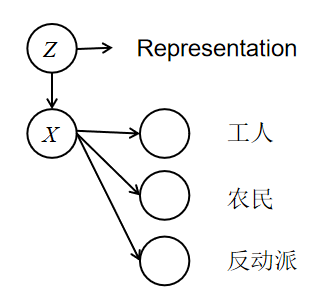
\includegraphics[width=.35\textwidth]{微信图片_20200627152457.png}
    \caption{GMM分类示意图}
    \label{fig:my_label_1}
\end{figure}
\textbf{那么,怎样才可以增加$Z$的特征信息呢?因为$Z$是离散的一维的隐变量,那么把它扩展成离散的高维的随机变量,不就行了。}那么,变化就来了,大家看好了。GMM中$Z$是离散的一维变量,那么在VAE被扩展为$m$维的高斯分布$Z\sim \mathcal{N}(0,I_{m\times m})$。而在给定$Z$的条件下,$P(X|Z)\sim \mathcal{N}(\mu_{\theta}(Z),\sum_{\theta}(Z))$。这里采用神经网络来逼近均值和方差,而不通过重参数化技巧这些直接去算(太麻烦了)。那么均值和方差是一个以$Z$为自变量,$\theta$为参数的函数。那么,假设条件可以总结为:
\begin{equation}
    \left\{
    \begin{array}{ll}
        Z\sim \mathcal{N}(0,I_{m\times m}) &  \\
        P(X|Z)\sim \mathcal{N}(\mu_{\theta}(Z),\sum_{\theta}(Z)) & 
    \end{array}
    \right.
\end{equation}
其中$Z\sim \mathcal{N}(0,I_{m\times m})$是一个先验分布假设,$Z$服从怎样的先验分布都没有关系,只要是高维的连续的就行了,只是在这里假设为Gaussian。我们关心的不是先验,我们实际上关心的是后验$P(Z|X)$,$Z$实际上只是帮助我们建模的。那么,接下来可以做一系列的推导:
\begin{equation}
    P_\theta(X) = \int_Z P_\theta(X,Z)dZ = \int_Z P(Z)P_\theta(X|Z) dZ
\end{equation}
推导到了这里有个什么问题呢?因为$Z$是一个高维的变量,所以$\int_z P(Z)P_\theta(X|Z) dZ$是intractable,积分根本算不出来。由于,$P_\theta(X)$是intractable,直接导致$P_\theta(Z|X)$也算不出来。因为根据Bayesian公式,
\begin{equation}
    P_\theta(Z|X) = \frac{P_\theta(Z)P_\theta(X|Z)}{P_\theta(X)}
\end{equation}
\textbf{实际上这里就是贝叶斯推断中一个很常见的现象,即为归一化因子计算困难。}

本小节主要从建模的角度介绍了VAE,实际上这就是一个Latent Variable Model。而GMM是$k$个离散的高斯分布的组合,由于隐变量$Z$是一维的离散变量,所以表达能力有限。为了增加其泛化能力,将其扩展为高维连续的变量。又因为其维度过高,导致通常情况下,后验分布基本是intractable。所以,下一小节将介绍如何求解此类问题。

\section{VAE的推断和学习}
上一小节中简要的描述了VAE的模型表示,下图则是VAE的模型图。
\begin{figure}[H]
    \centering
    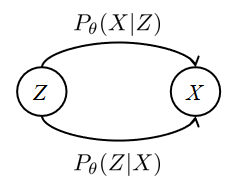
\includegraphics[width=.25\textwidth]{微信图片_20200627160913.png}
    \caption{VAE简单示意图}
    \label{fig:my_label_1}
\end{figure}
假设$\theta$这些都已经求出来了。如果要生成一个样本,怎么生成呢?我们先从$Z\sim P(Z)$中进行采样得到一个$z^{(i)}$。那么,$x^{(i)}\sim P_\theta(X|Z=z^{(i)})$进行采样即可。所以,这下大家可以深刻的理解,为什么我们关注的是后验$P(X|Z)$了。而$P_\theta(X|Z=z^{(i)})$是什么?我们用一个神经网络取逼近它就行了。\textbf{注意:本文中将其假设为高斯分布,并不是必要的,这个都是我们自定义的,是不是高斯分布都没有关系。}由于$P\theta(X|Z)$是intractable的,所以自然的想到可以用一个简单分布去逼近它:$Q_\phi(Z|X) \to P\theta(X|Z)$,即为:
\begin{figure}[H]
    \centering
    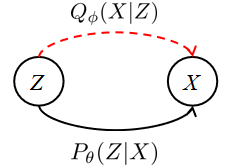
\includegraphics[width=.25\textwidth]{微信图片_20200627163051.png}
    \caption{VAE的变分推断法简单示意图}
    \label{fig:my_label_1}
\end{figure}
前面已经讲过很多遍了,通常方法可以将$\log P(X)$做如下分解:
\begin{equation}
    \log P(X)=\text{ELBO}+\text{KL}\left(Q_{\phi}(Z \mid X) \| P_{\theta}(Z \mid X)\right)
\end{equation}
然后采用EM算法求解,EM算法是一种基于时间的迭代算法,之前已经做了详细的解释,大家可以自行查阅,

E-step为:当$Q=P_\theta(Z|X)$时,KL=0,此时expectation就是ELBO。

M-step为:
\begin{equation}
    \theta = \arg\max_\theta \text{ELBO} = \arg\max_\theta \mathbb{E}_{P_\theta(Z
    |X)}[\log P_\theta(X,Z)]
\end{equation}
但是,肯定EM算法是用不了的,原因很简单$Q=P_\theta(Z|X)$这一步根本就做不到,$P_\theta(Z|X)$求不出来的。我们的求解目标是使$P_\theta(Z|X)$和$Q_\phi(Z|X)$靠的越近越好。那么可以表达为:
\begin{equation}
    \begin{split}
        \langle \hat{\theta}, \hat{\phi} \rangle = & \arg\min \text{KL}(Q_\phi(Z|X) \|P_\theta(Z|X) ) \\
        = & \arg\max \text{ELBO} \\
        = & \arg\max \mathbb{E}_{Q_\theta(Z|X)}[\log \underbrace{P_\theta(X,Z)]}_{P_\theta(X|Z)P(Z)} + \text{H}(Q_\phi(Z|X)) \\
        = & \arg\max \mathbb{E}_{Q_\theta(Z|X)}[\log P_\theta(X|Z)] - \text{KL}(Q_\phi(Z|X) \|P_\theta(Z)) \\
    \end{split}
\end{equation}
然后,关于$\theta$和$\phi$求梯度,采用梯度上升法来求解最优参数。可能大家会看到很多的叫法,SGVI,SGVB,SVI,Amortized Inference,实际上都是一样的,都是结合概率图模型和神经网络,使用重参数化技巧来近似后验分布,至于梯度怎么求,在“变分推断”中详细的介绍了SGVI方法的梯度计算方法。而怎样从分布$Q_\phi(Z|X)$中进行采样呢?用到的是重参数化技巧。
\begin{figure}[H]
    \centering
    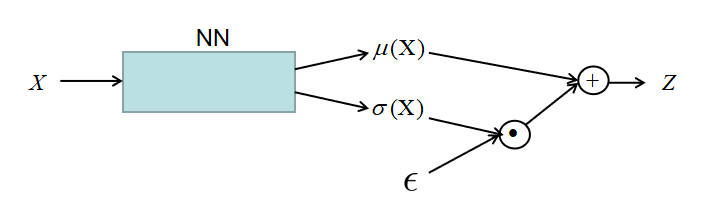
\includegraphics[width=.75\textwidth]{微信图片_20200627182516.png}
    \caption{VAE的求解过程简单示意图}
    \label{fig:my_label_1}
\end{figure}
其中,$\epsilon$是噪声,通常假定为$\epsilon \sim \mathcal{N}(0,I)$;而且,$P(Z|X) \sim \mathcal{N}(\mu_\phi(X),\sum_\phi(X))$,而很容易可以得到,$Z = \mu_\phi(X) + \sum_\phi(X)^{\frac{1}{2}}\cdot \epsilon$。那么到这里就基本思想就讲完了,想了解更多的东西,建议看看苏建林的blog:\url{https://spaces.ac.cn/}。

实际上大家会发现,所谓的VAE不过是“新瓶装旧酒”。只不过是用之前的技术对当前的概念进行了包装而已。大家可以关注一下这两项,$\mathbb{E}_{Q_\phi(Z|X)}[\log P_\theta(X|Z)]$和$\text{KL}(Q_\phi(Z|X) \|P_\theta(Z))$。这个$Z\to X$的过程可以被称为Decode,而$X \to Z$被称为Encode。我们可以看到,在训练过程中,首先是从$Q_\phi(Z|X)$中采样得到$z^{(i)}$:$z^{(i)} \sim Q_\phi(Z|X)$,然后利用$z^{(i)}$生成出样本$x^{(i)}$,即为$x^{(i)} = X \sim P(X|Z=z^{(i)})$。这样就形成了一个环,从$X$开始到$X$结束。\textbf{注意:训练时,$Z$由$Q_\phi(Z|X)$生成,而生成样本时,$Z$是从简单的高斯分布中采样得到的。}

而$\text{KL}(Q_\phi(Z|X) \|P_\theta(Z))$就是一个正则化项,对$Q_\phi(Z|X)$有一个约束,希望其尽量靠近标准高斯分布。不让模型坍缩到一个点上,如果没有这一项,只是去学习$\mathbb{E}_{Q_\phi(Z|X)}[\log P_\theta(X|Z)]$就很有可能会过拟合。第一项应该是真正的objective function,而第二项是一个regularization。实际上第二项扮演的功能和熵正则化项是一样的,都是使分布尽可能均匀,从而保留更多的可能性,因为熵就是信息量的表现,熵越大可能性越大。

以上就是对公式(6)中结果的详细解释。

\section{小结}
本节只是对VAE的简单描述,更深层次的思想可以参考苏建林的blog:\url{https://spaces.ac.cn/}。本节主要介绍了VAE的模型表示和推断学习过程。有关变分推断的部分,请大家自行阅读“变分推断”中的SGVI方法和“近似推断”那一小节,其中都做了详细的描述。我觉得本章的可读点在,1.从GMM模型中引出了VAE,VAE不过是GMM的进阶版。2.进阶以后发现维度太高,后验分布$P_\theta(Z|X)$计算不出来,于是采用简单分布$Q_\phi(Z|X)$来近似,这就变分法的思想。3.详细的介绍了优化ELBO中每一项的意思,这里$\text{KL}(Q_\phi(Z|X) \|P_\theta(Z))$是正则化项,相信很多同学在看VAE中,描述令表示层服从高斯分布的时候都是一脸懵逼的吧。4.本文中还复习了用神经网络,代替分布进行采样的重参数化技巧。

其实VAE不过是“新瓶装旧酒”,本身并没有什么技术的革新,用到的算法和思想都是比较老的。

\end{document}
